%========================================================================================
% Compilation should work with PDFLaTeX
%========================================================================================
% Type of document and general formatting
\documentclass[a4paper,11pt]{article}

\usepackage[left=2.5cm,right=2.5cm,top=2.5cm,bottom=2.5cm]{geometry}
\linespread{1.25}

%========================================================================================
% These packages are for language and font settings
\usepackage[english,activeacute]{babel} % Language
\usepackage{tgpagella}					% Text font
\usepackage[T1]{fontenc}				% T1 Encoding of font
\usepackage[utf8]{inputenc}				% Special symbols
\usepackage{lmodern}


%========================================================================================
\usepackage[sc]{mathpazo}				% Math font
\usepackage{amsmath,amsfonts,amssymb}	% Math symbols
\usepackage{dsfont}						% Math symbols like R for reals...
\usepackage{amsthm}						% For theorem styles
\usepackage{siunitx}

%========================================================================================
% Other packages
\usepackage{graphicx}
\usepackage{longtable}
\usepackage[svgnames]{xcolor}

%========================================================================================
\usepackage{accents}
\newcommand*{\dt}[1]{%
	\accentset{\mbox{\large\bfseries .}}{#1}} % Larger dot for time derivative


\usepackage{hyperref}
\hypersetup
{
    pdfauthor={Rafael Serrano-Quintero},
    pdfsubject={Structural Transformation in Indian Services},
    colorlinks = {true},
    linkcolor = {FireBrick},
    citecolor = {FireBrick},
    urlcolor = {RoyalBlue},
}

\usepackage{appendix}
\usepackage{marvosym}
\usepackage{enumerate} %For enumerating with letters with option [a)]
\usepackage{enumitem}
\usepackage{fancyvrb}  %To reduce font size in verbatim environment
\usepackage{epstopdf}
\usepackage[flushleft]{threeparttable}
\usepackage{pdflscape}
\usepackage{natbib}
\usepackage{subcaption}
\usepackage{booktabs}
\usepackage[super]{nth}
\usepackage{float}

\newcommand{\source}[1]{\caption*{\tiny Source: {#1}} }

%========================================================================================
% Stata Preamble for Tables
%========================================================================================

\newcommand{\sym}[1]{\rlap{#1}}% Thanks to David Carlisle

\let\estinput=\input% define a new input command so that we can still flatten the document

\newcommand{\estwide}[3]{
		\vspace{.75ex}{
			\begin{tabular*}
			{\textwidth}{@{\hskip\tabcolsep\extracolsep\fill}l*{#2}{#3}}
			\toprule
			\estinput{#1}
			\bottomrule
			\addlinespace[.75ex]
			\end{tabular*}
			}
		}	

\newcommand{\estauto}[3]{
		\vspace{.75ex}{
			\begin{tabular}{l*{#2}{#3}}
			\toprule
			\estinput{#1}
			\bottomrule
			\addlinespace[.75ex]
			\end{tabular}
			}
		}

% Allow line breaks with \\ in specialcells
	\newcommand{\specialcell}[2][c]{%
	\begin{tabular}[#1]{@{}c@{}}#2\end{tabular}}

% *****************************************************************
% Custom subcaptions
% *****************************************************************
% Note/Source/Text after Tables
\newcommand{\figtext}[1]{
	\vspace{-1.9ex}
	\captionsetup{justification=justified,font=footnotesize}
	\caption*{\hspace{6pt}\hangindent=1.5em #1}
	}
\newcommand{\fignote}[1]{\figtext{\emph{Note:~}~#1}}

\newcommand{\figsource}[1]{\figtext{\emph{Source:~}~#1}}

% Add significance note with \starnote
\newcommand{\starnote}{\figtext{* p < 0.1, ** p < 0.05, *** p < 0.01. Standard errors in parentheses.}}

% *****************************************************************
% siunitx
% *****************************************************************
\usepackage{siunitx} % centering in tables
	\sisetup{
		detect-mode,
		tight-spacing           = true,
		group-digits            = false ,
		input-signs             = ,
		input-symbols           = ( ) [ ] - + *,
		input-open-uncertainty  = ,
		input-close-uncertainty = ,
		table-align-text-post   = false
        }

% Document parameters
\title{Chapter 3: Integral Calculus}
\author{Rafael Serrano Quintero \\
Dpt. Fundamentos del An\'alisis Econ\'omico \\
University of Alicante}
\date{}

\theoremstyle{definition}
\newtheorem{definition}{Definition}
\newtheorem{property}{Property}
\newtheorem{example}{Example}
\newtheorem{remark}{Remark}
\theoremstyle{plain}
\newtheorem{theorem}{Theorem}
\newtheorem{lemma}{Lemma}
%========================================================================================
					% === Title, thanks, and author data === %
%========================================================================================

\begin{document}      

\maketitle

\section{The Area Problem}\label{the-area-problem}

Suppose that we have a (inverse) demand function such as \(p = f(q)\) relating price \((p)\) and quantity \((q)\) of a commodity. Let us assume that the commodity is something like a house or a car, so that consumers will only buy one unit of \(Q\). We can think of the demand function \(q = f^{-1}(p)\) as counting how many consumers have reservation price larger than or equal to \(p\). Figure \ref{fig:area_under_curve} shows the graph of the inverse demand function.

\begin{figure}[htbp]
	\centering 
 		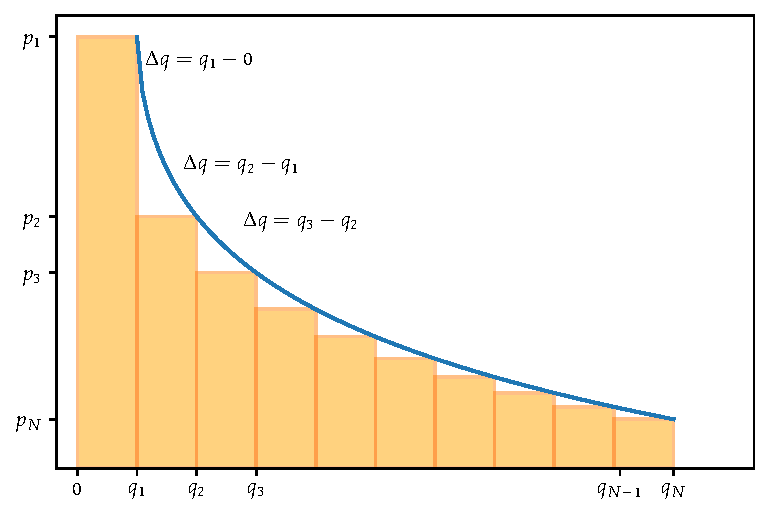
\includegraphics[width = 0.8\textwidth]{Ch3_files/Ch3_3_0.pdf}
		\caption{}
		\label{fig:area_under_curve}
\end{figure}
    
To compute the consumer's total willingness to pay for \(Q\), let's assume that the producers of \(Q\) sell it in small lots \(\Delta q = q_{n} - q_{n-1}\) with \(q_n = n\Delta q\) for any \(n = 1,2,\ldots,N\). By selling at price \(p_1\) the producer can sell
the first lot, and consumer expenditure will be equal to \(q_1 \cdot p_1 = (q_1-0)\cdot f(q_1)\). The second lot would be sold at a price of \(p_2\) and thus, now total consumer expenditure would be equal to \(f(q_1)(q_1 - 0) + f(q_2)(q_2 - q_1)\) which is the area of the two first rectangles in Figure \ref{fig:area_under_curve}. This can go on at each step, at the end, total consumer expenditure is

\[
\sum^N_{n=1} f(q_n)(q_n - q_{n-1})
\]

This is the \textbf{Riemann sum} of the inverse demand function in Figure \ref{fig:area_under_curve}. However, notice that we have made the assumption that producers can only sell in \emph{small lots}. In the actual market, only \(q^*\) units will be sold at a price \(p^*\) and thus, the area under the curve from \(q = 0\) up to \(q = q^*\) is
sometimes called the \textbf{total willingness to pay} for \(q^*\) units. Total willingness to pay minus actual expenditure (in equilibrium, actual expenditure is \(q^* f(q^*)\)) is called the \textbf{consumer surplus}.

If instead we would assume that the commodity is well approximated by a continuous variable \(q\) (e.g.~massages, and \emph{producers} sell whatever amount of time of massage) this process of adding up the areas of the rectangles would be missing the little white spaces in between the curve and the rectangles. One of the possibilities is to make the rectangles thinner and thinner but this will only give us an approximation or some bounds for this area. If we could make the width of the rectangles infinitesimally small and then we could compute the sum, then it would no longer be an approximation but the actual value of the area under the curve. Formally, the area under the inverse demand curve is given by

\[
\lim_{n\rightarrow \infty} \sum^n_{i=1} f(q_i)(q_i-q_{i-1})
\]

We are at a point where we can define the \textbf{definite integral}.

\begin{definition}
If \(f\) is a function defined for \(a\leq x \leq b\), we divide the interval \([a,b]\) into \(n\) subintervals of equal width \(\Delta x = (b-a)/n\). Letting \(x_0 = a\) and \(x_n = b\) be the initial and ending points of the interval, and \(x_i^*\) for \(i=1,2,\ldots,n\) be any points inside these subintervals, so that \(x_i^*\in[x_{i-1},x_i]\). Then, the \textbf{definite} integral of \(f\) from \(a\) to \(b\) is

\[
\int^b_a f(x) dx = \lim_{n\rightarrow\infty} \sum_{i=1}^n f(x_i^*)\Delta x
\]

provided that this limit exists. If it does exist, we say \(f\) is \textbf{integrable} on \([a,b]\).
\end{definition}

\begin{remark}
The precise meaning of this limit is that

\(\forall\varepsilon > 0 \ \exists N\in\mathbb{Z} \ : \ \) 

	\[
    \Bigg\lvert \int^b_a f(x) dx - \sum_{i=1}^n f(x_i^*)\Delta x \Bigg\rvert < \varepsilon
    \]

\(\forall n > N\) and for every choice of \(x_i^*\in[x_{i-1}, x_i]\)
\end{remark}

\begin{remark}
An important assumption we have made is that we are talking about \textbf{positive} functions, which makes sense for demand functions since we only care about positive quantities of goods. However, if we had a function that would take positive and negative
values, then the Riemann sum would correspond to the sum of the areas of the rectangles that lie above the \(x-\)axis and the negatives of the areas of the rectangles that lie below the \(x-\)axis.
\end{remark}

An issue that we have not talked about yet is whether the limit that
defines the definite integral exists or not and under which conditions.
We state an important theorem about this.

\begin{theorem}
If \(f\) is a continuous function on \([a,b]\), or if \(f\) has only a finite number of jump discontinuities, then \(f\) is integrable on \([a,b]\); i.e., the definite integral \(\int^b_a f(x) dx\) exists.
\end{theorem}


\begin{example}
Evaluate the Riemann sum for \(f(x) = x^3 - 6x\) in \([0,3]\) with \(6\) intervals.

\begin{enumerate}
\item Interval width is given by \(\Delta x = (3-0)/ 6 = 1/2\)
\item Let's take the right-end points as our \(x_i\). That is the points \(\{0.5, 1, 1.5, 2, 2.5, 3\}\)
\item The Riemann sum is then:
\begin{align*}
f(0.50) &= -2.875 \\
f(1.00) &= -5.000 \\
f(1.50) &= -5.625 \\
f(2.00) &= -4.000 \\
f(2.50) &=  0.625 \\
f(3.00) &=  9.000 \\
\sum^6_{i=1} f(x_i)\Delta x &= \Delta x \sum^{6}_{i=1}f(x_i) = -3.9375
\end{align*}

\end{enumerate}
\end{example}

\begin{example}
Evaluate now \(\displaystyle\int^3_0 (x^3-6x) dx\).

\begin{enumerate}
\item Note first that with \(n\) subintervals, \(\Delta x = 3/n\).
\item The lower bound of the interval is \(0\), thus \(x_0 = 0, x_1 = 3/n, x_2 = 6/n,\ldots, x_i = (3i)/n\).
\item Now we can use these as our sample points.
\end{enumerate}

\begin{align*}
\int^3_0 (x^3-6x) dx &= \lim_{n\rightarrow\infty} \sum^n_{i=1} f(x_i) \Delta x = \lim_{n\rightarrow\infty} \sum^n_{i=1} f\left(\frac{3i}{n}\right) \frac{3}{n} \\
&= \lim_{n\rightarrow\infty} \frac{3}{n} \sum^n_{i=1} \left[\left(\frac{3i}{n}\right)^3 - 6\left(\frac{3i}{n}\right)\right] = \lim_{n\rightarrow\infty} \frac{3}{n} \sum^n_{i=1} \left[ \frac{27i^3}{n^3} - \frac{18 i}{n} \right] \\
&= \lim_{n\rightarrow\infty} \left[\frac{81}{n^4} \sum^n_{i=1} \left(i^3\right) - \frac{54}{n^2} \sum^n_{i=1} \left(i\right)\right] = \lim_{n\rightarrow\infty} \left[\frac{81}{n^4} \left(\frac{n(n+1)}{2}\right)^2 - \frac{54}{n^2} \left(\frac{n(n+1)}{2}\right)\right] \\
&= \lim_{n\rightarrow\infty} \left[\frac{81}{4} \left(\frac{n(n+1)}{n^2}\right)^2 - 27\left(\frac{n(n+1)}{n^2}\right)\right] \\
&= \lim_{n\rightarrow\infty} \left[\frac{81}{4} \left(1+\frac{1}{n}\right)^2 - 27\left(1+\frac{1}{n}\right)\right] = \frac{81}{4} - 27 = \frac{-27}{4} = -6.75
\end{align*}

The results are strikingly different, since \(n = 6\) is a poor approximation for the Riemann sum to equal the definite integral. Note further, this cannot be interpreted as an area since the function takes on negative values. Figure \ref{fig:riemann_vs_actual} shows why \(n=6\) yields a poor result.
\end{example}

 \begin{figure}[htbp]
 	\centering 
 		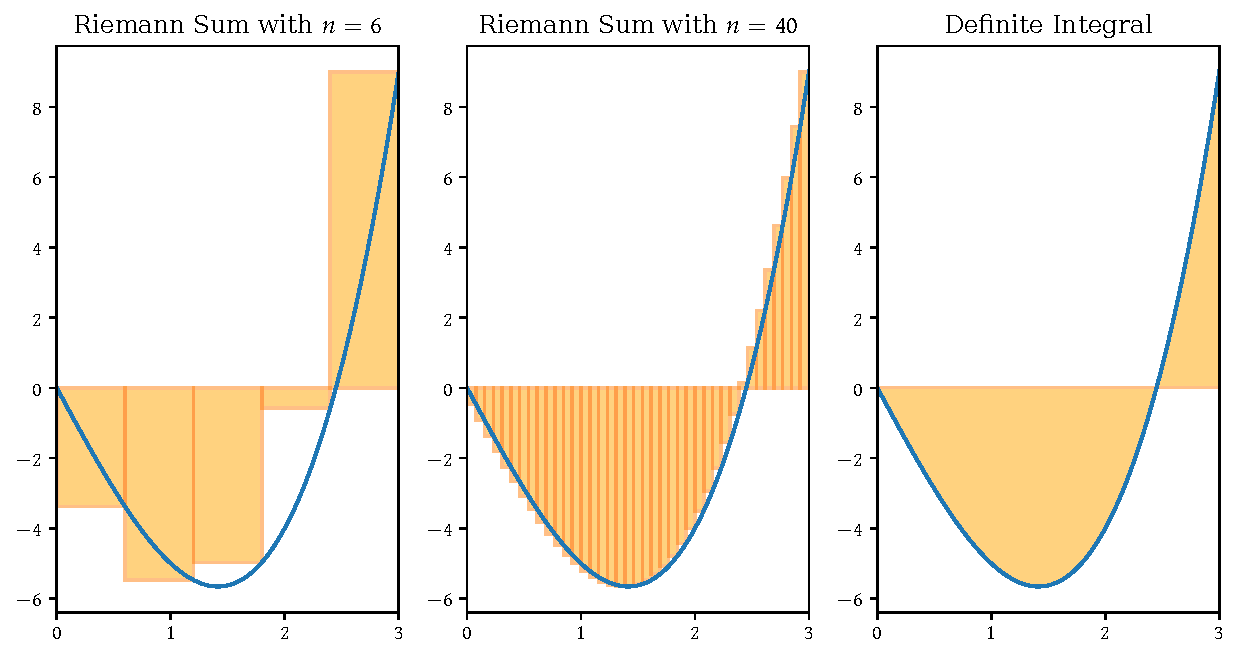
\includegraphics[width = 0.8\textwidth]{Ch3_files/Ch3_7_0.pdf}
 		\caption{}
 		\label{fig:riemann_vs_actual}
 \end{figure}
    
\section{The Fundamental Theorem of Calculus}\label{the-fundamental-theorem-of-calculus}

This theorem is so important (fundamental) because it stablishes the connection between two branches of calculus, differential and integral calculus. Isaac Barrow (Newton's mentor) discovered how the area problem and the tangent problem are related, in fact, he discovered that integration and differentiation are inverse processes. Before getting into the theorem itself, let us start by giving some definitions.

\begin{definition}
Given a function \(f(x)\) it is called a \textbf{primitive} (or \textbf{indefinite integral}) to another function \(F(x)\) such that

\[
F'(x) = f(x)
\]

\end{definition}

\begin{example}
Take \(f(x) = 2x\). Then: 

\begin{enumerate}
	\item \(F(x) = x^2 - \pi\) is a primitive. 
	\item \(F(x) = x^2 + 2\) is a primitive. 
	\item \(F(x) = x^2 - 73\) is a primitive. 
	\item \(F(x) = x^2 + \mathcal{C}\) is a primitive \(\forall C\in\mathbb{R}\)
\end{enumerate}
\end{example}

Therefore, two primitives of a function differ \textbf{only} by a constant. Let \(F(x)\) and \(G(x)\) be two primitives of a function \(f(x)\), then

\[
F'(x) = G'(x) = f(x) \ \Rightarrow \ \left(F(x)-G(x)\right)' = 0 \ \Rightarrow \ F(x) - G(x) = \mathcal{C}
\]

The set of all primitives of a function \(f(x)\) is denoted by \(\displaystyle\int f(x) dx\).

\begin{remark}
It is very important to notice that a definite integral is a \textbf{number} while an indefinite integral is a \textbf{family of functions}. They are \textbf{not} the same thing.
\end{remark}

\textbf{Immediate Primitives:} These are directly obtained from the
differentiation rules.

\begin{itemize}
	\item $\displaystyle\int x^r dx = \dfrac{x^{r+1}}{r+1} + \mathcal{C}, \quad r \neq -1$
	\item $\displaystyle\int x^{-1} dx = \displaystyle\int \dfrac{1}{x} dx = \ln(x) + \mathcal{C}$
	\item $\displaystyle\int e^x dx = e^x + \mathcal{C}$
	\item $\displaystyle\int \cos(x) dx = \sin(x) + \mathcal{C}$
	\item $\displaystyle\int \sin(x) dx = -\cos(x) + \mathcal{C}$
	\item $\displaystyle\int \frac{1}{1+x^2} dx = \arctan(x) + \mathcal{C}$
\end{itemize}


\subsection{Properties of Integrals}\label{properties-of-integrals}

\paragraph{Linearity}\label{linearity}

We know that the derivative of the sum of two functions is the sum of the derivatives and that the derivative of a constant multiplied by a function is just the constant multiplied by the derivative of the function. These linearity properties carry over to the process of integration.

\begin{enumerate}
\item \(\displaystyle\int k f(x) dx = k \displaystyle\int f(x) dx\)
\item \(\displaystyle\int (f(x) + g(x)) dx = \displaystyle\int f(x) dx + \displaystyle\int g(x) dx\)
\end{enumerate}

\paragraph{Substitution}\label{substitution}

This property is based on the derivative of a composite function, that is, suppose we have \(f(x) = \log(\sin(x))\), letting \(z = \sin(x)\) the derivative of \(f(z)\) is given by

\[
f'(z) = \frac{dz}{z} = \frac{\cos(x)}{\sin(x)}
\]

Using the same argument in integration, if

\[
\int f(x) dx = F(x) \Rightarrow \int f(z) dz = F(z)
\]

Basically, \emph{we do not care about the name of the variable} to obtain the primitive of the function.

\begin{example}
Integrate: 

$$
\int 2 e^{2x} dx = \int e^{2x}d(2x) = \int e^z dz = e^z + \mathcal{C} = e^{2x} + \mathcal{C}
$$
\end{example}

\textbf{Some other Immediate Primitives:}
\begin{itemize}
	\item $\displaystyle\int [f(x)]^r f'(x) \: dx = \dfrac{[f(x)]^{r+1}}{r+1} + \mathcal{C}, \quad r \neq -1$
	\item $\displaystyle\int \dfrac{f'(x)}{f(x)} \: dx = \ln(f(x)) + \mathcal{C}$
	\item $\displaystyle\int f'(x) e^{f(x)} \: dx = e^{f(x)} + \mathcal{C}$
	\item $\displaystyle\int \cos(f(x))f'(x) \: dx = \sin(f(x)) + \mathcal{C}$
	\item $\displaystyle\int \sin(f(x)) f'(x) \: dx = -\cos(f(x)) + \mathcal{C}$
	\item $\displaystyle\int \dfrac{f'(x)}{1+[f(x)]^2} \: dx = \arctan(f(x)) + \mathcal{C}$
\end{itemize}

\subsection{The Fundamental Theorem of Calculus. Part I}\label{the-fundamental-theorem-of-calculus.-part-i}

Before stating and proving Part I of the Fundamental Theorem of Calculus, let us state and prove one important property of integrals.

\begin{property}\label{bounds}
If \(m\leq f(x) \leq M\) for \(a\leq x \leq b\), then:

\[
m(b-a) \leq \int^b_a f(x) dx \leq M(b-a) 
\]
\end{property}

\begin{theorem}{\textbf{The Fundamental Theorem of Calculus, Part I:}}\label{thm:FTC1}
If \(f\) is continuous on \([a,b]\), then the function \(g\) defined by

\[
g(x) = \int^x_a f(t) dt
\]

for \(a\leq x \leq b\) is continuous on \([a,b]\) and differentiable on \((a,b)\), and \(g'(x) = f(x)\)
\end{theorem}


\begin{proof}
If \(x\) and \(x+h\) are in \((a,b)\) then:

\begin{align*}
g(x+h) - g(x) &= \int^{x+h}_a f(t) dt - \int^x_a f(t) dt \\
&= \left(\int_a^x f(t) dt + \int_x^{x+h} f(t)dt\right) - \int^x_a f(t) dt \\
&= \int_x^{x+h} f(t)dt 
\end{align*}

And so, for \(h\neq 0\):

\begin{equation}
\frac{g(x+h)-g(x)}{h} = \frac{1}{h}\int_x^{x+h} f(t) dt
\label{eqn:important_eqn_FTC1}
\end{equation}

Let us assume that \(h>0\) by now. Since \(f(x)\) is continuous on \([x,x+h]\), Weierstrass' Theorem tells us that there are two numbers \(u,v\in[x,x+h]\) such that \(f(u) = m\) and \(f(v) = M\) where \(m\) and \(M\) are the absolute minimum and maximum values of \(f\) on \([x,x+h]\). By Property \ref{bounds}, we have

\[
mh \leq \int^{x+h}_x f(t) dt \leq Mh
\]

\[
f(u)h \leq \int^{x+h}_x f(t) dt \leq f(v) h
\]

Since \(h>0\) we can divide by \(h\):

\[
f(u) \leq \frac{1}{h}\int^{x+h}_{x}f(t) dt \leq f(v)
\]

Replacing Equation \eqref{eqn:important_eqn_FTC1}:

\[
f(u) \leq \frac{g(x+h)-g(x)}{h} \leq f(v)
\]

Let now \(h\rightarrow 0\). Then, both \(u\) and \(v\) tend to \(x\) since they are inside \([x,x+h]\). Therefore:

\begin{align*}
\lim_{h\rightarrow 0} f(u) &= \lim_{u\rightarrow x} f(u) = f(x) \\
\lim_{h\rightarrow 0} f(v) &= \lim_{v\rightarrow x} f(v) = f(x) 
\end{align*}

Then, using the last inequality from before:

\begin{equation}
g'(x) = \lim_{h\rightarrow 0} \frac{g(x+h)-g(x)}{h} = f(x)
\label{eqn:FTC_proof}
\end{equation}

If \(x = a\) or \(x = b\), then equation \eqref{eqn:FTC_proof} is interpreted as a one-side limit. Since \(g(x)\) is differentiable on \([a,b]\) then \(g(x)\) is continuous on \([a,b]\).
\end{proof}

\begin{example}
Let us use an example where we can use the Fundamental Theorem of Calculus. 
\begin{enumerate}
	\item Draw the graph of the function \(f(x) = \cos(x^2)\) in the rectangle \([0, 2]\times[-1.25, 1.25]\). 
	\item Define now 
			\[
			g(x) = \int^x_0 \cos(t^2) dt
			\] 

	\(g(x)\) is now the area under the graph of \(f(x)\) up to the point where it becomes a difference of areas (when \(f(x)<0\)). 
	\item Use \(g(x)\) to estimate the areas by computing \(g(0.2), g(0.4),\ldots,g(1.8),g(2)\).

	\begin{align*}
		g(0.20) &= 0.20 \ & \ g(0.40) &= 0.40 \\
		g(0.60) &= 0.59 \ & \ g(0.80) &= 0.77 \\
		g(1.00) &= 0.90 \ & \ g(1.20) &= 0.97 \\
		g(1.40) &= 0.95 \ & \ g(1.60) &= 0.83 \\
		g(1.80) &= 0.64 \ & \ g(2.00) &= 0.46
	\end{align*}

	Just by computing g(x) we can see that for some \(x\in[1.20, 1.40]\) \(f(x)\) will become zero, and afterwards, negative since \(g(x)\) has declined. Furthermore, we observe that from \(x = 0\) up to \(x = 0.6\) \(g(x)\) increases the same amount and \(g(x)\) is increasing up to \(x = 1.20\). This tells us that the function is approximately constant for \(x\in[0,0.6]\) and \(f(x) > 0\) for \textbf{at least} those \(x\in[0, 1.20]\). We know that for \(x > 1.20\) the function becomes negative.

	\item The graph of \(g'(x)\) would be now \(f(x)\), we can infer the graph of \(g'(x)\) from the definition of the derivative (the slope of a tangent line).
\end{enumerate}

Figure \ref{fig:ftc_illustration} shows both the graph of $f(x)$ and the values of $g(x)$ we have computed.
\end{example}

\begin{figure}[htbp]
	\centering 
		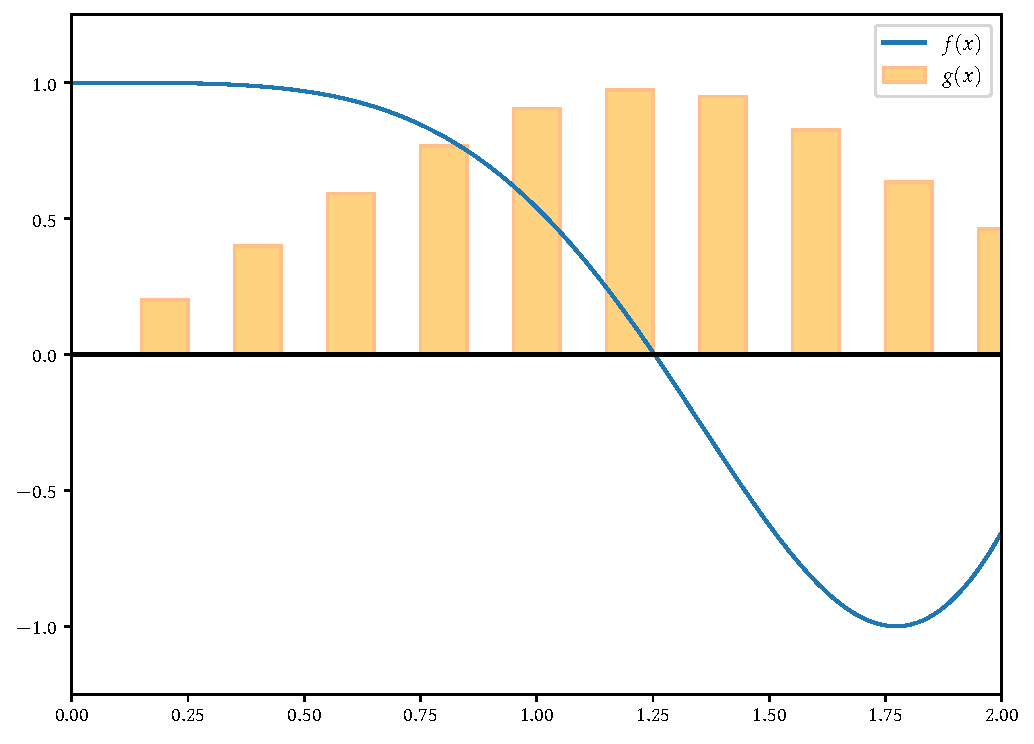
\includegraphics[width = 0.8\textwidth]{Ch3_files/Ch3_14_0.pdf}
	\caption{}
	\label{fig:ftc_illustration}
\end{figure}

    
\begin{example}
Find 

\[
\frac{d}{dx}\int^{x^4}_1 cos(t) dt
\]

Let \(u = x^4\). 

\begin{align}
	\frac{d}{dx}\int^{x^4}_1 cos(t) dt &= \frac{d}{dx}\int^{u}_1 cos(t) dt & \  & \\
	&= \frac{d}{du}\left(\int^{u}_1 cos(t) dt\right)\frac{du}{dx} & \  & \ \text{by the Chain Rule} \\
	&= cos(u)\frac{du}{dx} & \ & \ \text{(by FTC Part 1)} \\
	&= cos(x^4)4x^3
\end{align}

We could also use the rules of integration and compute first \(\displaystyle\int^{x^4}_1 cos(t) dt\) and then differentiate the result with respect to \(x\).

  \[
  \int^{x^4}_1 cos(t) dt = \sin{\left(x^{4} \right)} - \sin{\left(1 \right)}
  \]   

  \[
  \frac{d}{dx}\int^{x^4}_1 cos(t) dt = \frac{d}{dx} \sin(x^4)-\sin(1) =  4 x^{3} \cos{\left(x^{4} \right)}
  \]
\end{example}


\subsection{The Fundamental Theorem of Calculus Part II}\label{the-fundamental-theorem-of-calculus-part-ii}

\paragraph{Recap}\label{recap}

So far, we have seen: 

\begin{itemize}
	\item The definite integral is related to the area problem. 
	\item The indefinite integral is the inverse operation of differentiation and thus it is related to the tangent problem. 
	\item Properties of integrals (linearity, substitution,...) 
	\item Fundamental Theorem of Calculus Part I (Theorem \ref{thm:FTC1}): If \(f\) is a continuous function on an interval, the function \(g(x) = \int^x_a f(t) dt\) is a primitive of \(f(x)\) and thus, \(g'(x) = f(x)\).
\end{itemize}

The second part of the Fundamental Theorem of Calculus is going to give us a way of computing definite integrals by using primitives.

\begin{theorem}{\textbf{Fundamental Theorem of Calculus, Part II:}} If \(f\) is
continuous on \([a,b]\), then

\[
\int^b_a f(x) dx = F(b) -  F(a)
\]

where \(F\) is any primitive of \(f\).
\end{theorem}

\begin{proof}
We know from FTC Part 1 that if \(g(x) = \int^x_a f(t) dt\) then, \(g'(x) = f(x)\); that is, \(g(x)\) is a primitive of \(f(x)\). Suppose now that \(F\) is any other primitive
of \(f\), then \(F(x) = g(x) + \mathcal{C}\), i.e., \(F\) and \(g\) differ only by a constant.

Computing now \(g(a)\):

\[
g(a) = \int^a_a f(x) dx = 0
\]

Then:

\begin{align*}
F(b) - F(a) & = \left(g(b)+\mathcal{C}\right) - \left(g(a)+\mathcal{C}\right)  \ & \ & \ \\
& = g(b) - g(a) = g(b) \ & \ & \  \\ \\
& = \int^b_a f(x) dx \ & \ & \ \text{by the definition of $g(x)$} 
\end{align*}
\end{proof}

\begin{remark}
The second part of the FTC tells us that we can compute the \textbf{exact} value of the integral \(\int^b_a f(x) dx\) if we know the value of a primitive at the two extremes of integration.
\end{remark}

\section{A Malthusian Model of Growth and Differential Equations}\label{a-malthusian-model-of-growth-and-differential-equations}

To illustrate how useful are integrals and differential equations, we are going to sketch a model of economic growth in terms of differential equations. The idea of the model goes back to Thomas Malthus and his hypothesis is that population and standards of living have been mostly constant throughout history because most of this time we had
\emph{agricultural societies}. If we suppose that output is produced using land and labor only and land is fixed, labor grows with births and declines with deaths but each additional worker increases production by less and less (diminishing returns). Since land is fixed, there is less and less land to work on for each of these additional workers. How does population increase? Population increases when people eat better and
there are better health conditions, thus, population growth is a function of output per capita. But when population grows, there is less land to work on, thus the increase in output is not sufficient to sustain the additional population, thus population declines. This tends to a constant population and output per capita.

Figure \ref{fig:gdppc_uk} shows GDP per capita in the United Kingdom since 1270 in the first panel. We observe it is mostly flat. The second panel of Figure \ref{fig:gdppc_uk} shows real GDP per capita and population levels for the world since 1870, we observe that they grow hand-in-hand.

 \begin{figure}[htbp]
 	\centering 
 		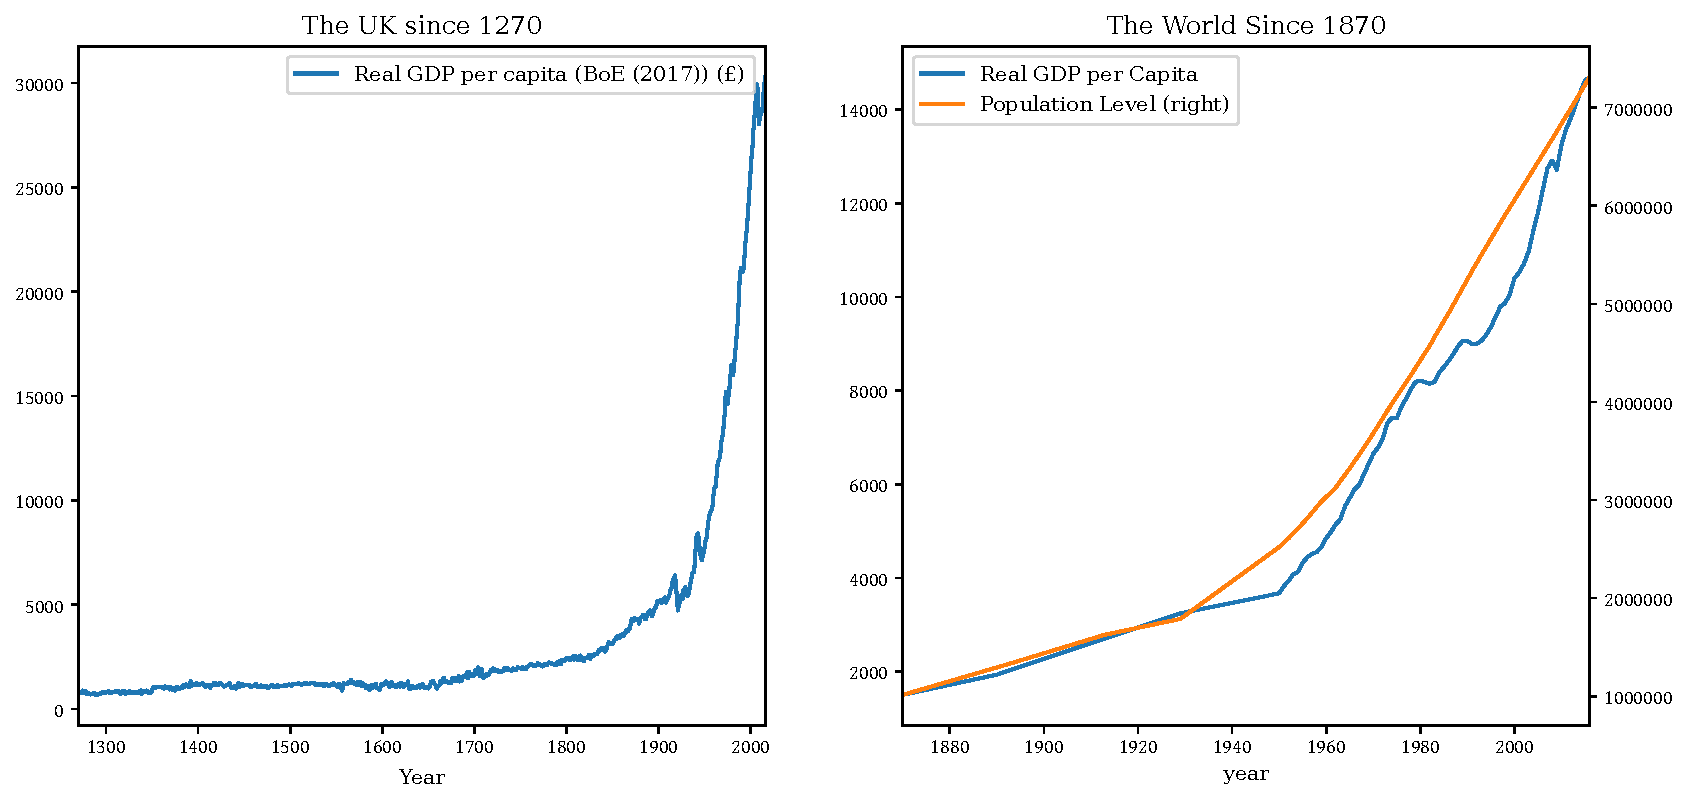
\includegraphics[width = 0.8\textwidth]{Ch3_files/Ch3_25_0.pdf}
 		\caption{}
 		\label{fig:gdppc_uk}
 \end{figure}
    

\subsection{The Simplest Malthusian Model of Growth}\label{the-simplest-malthusian-model-of-growth}

Suppose that output is produced using only land and labor as explained before, there is no technological progress and population grows as long as a minimum subsistence level of consumption is assured. Furthermore, land is fixed. The technology to produce output is given by

\[
Y = B X^{\beta}L^{1-\beta} \ ; \ 0 < \beta < 1
\]

Where \(Y\) is output, \(B\) is technological level (suppose this could change across countries but not \emph{within} countries), \(X\) is the stock of land (which is fixed), and \(L\) is labor. Income per capita is thus given by

\[
y \equiv \frac{Y}{L} = B\left(\frac{X}{L}\right)^{\beta}
\]

Note that as population grows, aggregate output grows but output \emph{per capita} falls. This is due to the diminishing returns to labor. More people try to work on the same stock of land available, thus there is a smaller piece of land for each additional worker.

Now, we define population growth as a function of output per capita, if output per capita rises, so does population. However, to have an increasing population, the economy must produce at least some subsistence term denoted \(\bar{c}\). Mathematically,

\[
\frac{\dot{L}}{L} = \theta\left(y - \bar{c}\right)
\]

Note that population growth can be negative, and it is likely that it will be negative since to increase we need to fulfill the subsistence requirement. Substituting the expression for output per capita:

\[
\frac{\dot{L}}{L} = \theta\left(B\left(\frac{X}{L}\right)^{\beta} - \bar{c}\right)
\]

This equation shows that population growth is inversely releated to population level. The larger it is population now, the lower will be its growth. This implies that when population levels are low, people is relatively rich, while for large populations, people tend to be poorer. This function is shown in Panel A of Figure \ref{fig:malthus_phase}.

 \begin{figure}[htbp]
 	\centering 
 		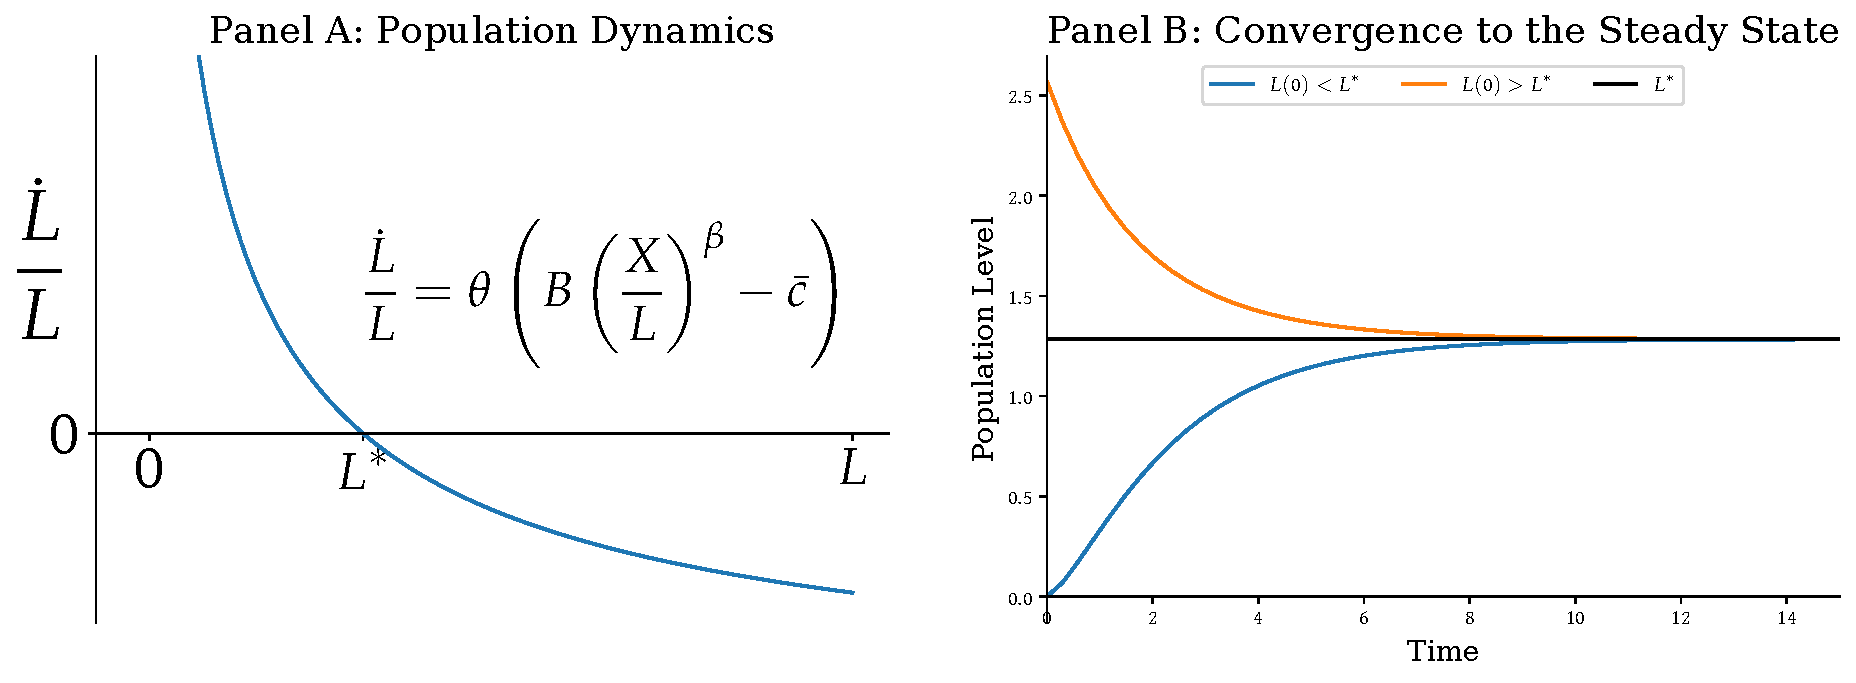
\includegraphics[width = 0.8\textwidth]{Ch3_files/Ch3_28_0.pdf}
 		\caption{}
 		\label{fig:malthus_phase}
 \end{figure}
    
Furthermore, the dynamics of this system ensure that the economy will always end up at \(L^*\) regardless of the starting point, as Panel B of Figure \ref{fig:malthus_phase} shows.

But, how can we actually use integrals to solve this differential equation? This example is a bit more complicated, let us simplify the model so that output is produced only using labor, \(Y = B L\), thus, output per capita is \(y = \frac{Y}{L}\) and therefore,

\[
\frac{\dot{L}}{L} = \theta\left(B - \bar{c}\right)
\]

To solve this differential equation, we can rewrite it so that

\[
\frac{dL}{dt} = \theta BL - \theta \bar{c} L = \theta L\left(B-\bar{c}\right)
\]

Since it is a separable equation, we divide on both sides by \(\theta L\left(B-\bar{c}\right)\) and integrate with respect to time \((t)\) to get the solution

\begin{align*}
\int \frac{\frac{dL}{dt}}{\theta\left(B-\bar{c}\right)L(t)} dt & = \int 1 dt \\
&= \int\frac{1}{\theta\left(B-\bar{c}\right)L(t)} = t + \mathcal{C} \\
&= \frac{\ln(L(t))}{\theta\left(B-\bar{c}\right)} = t + \mathcal{C} \\
&= L(t) = e^{\theta\left(B-\bar{c}\right)\left(t+\mathcal{C}\right)}
\end{align*}

The general solution of this differential equation depends on an arbitrary constant that will be determined depending on the initial condition of population level. Suppose \(L(0) = L_0\). Then, by substituting \(t = 0\) in the general solution and setting it equal to
\(L_0\), we get that

\[
\mathcal{C} = \frac{\ln\left(L_0\right)}{\theta\left(B-\bar{c}\right)}
\]

\begin{remark}
Can you tell whether this simplified economy is, in fact, Malthusian?
\end{remark}

Let us now solve the initial model. We start with the same steps as before by expressing the differential equation as

\[
\frac{dL}{dt} = \theta X^{\beta}L^{1-\beta} - \theta\bar{c}L
\]

It is again a separable equation, thus

\begin{align*}
\int \frac{\frac{dL}{dt}}{\theta X^{\beta}L^{1-\beta} - \theta\bar{c}L} dt &= \int 1 dt = t+\mathcal{C} & \ & \\
&= \int \frac{1}{\theta X^{\beta}L^{1-\beta} - \theta\bar{c}L} dL & \ & \\
&= \int \frac{L^{\beta-1}}{\theta X^{\beta} - \theta\bar{c}L^{\beta}} dL & \ & \text{(by multiplying and dividing by $L^{\beta-1}$)}
\end{align*}

It is convenient now to make a \textbf{change of variables}. Recall that when solving an integral we \emph{do not care about the name of the variable}, thus, let \(u = \theta X^{\beta} - \theta\bar{c}L^{\beta}\) and \(du = -\beta\theta\bar{c}L^{\beta-1}dL\). Therefore, we can solve the simpler integral

\[
-\frac{1}{\beta\theta\bar{c}}\int\frac{1}{u} du = -\frac{1}{\beta\theta\bar{c}}\ln(u) = -\frac{\ln\left(\theta X^{\beta} -\theta\bar{c}L^{\beta}\right)}{\beta\theta\bar{c}} = t+\mathcal{C}
\]

By exponentiating on both sides and solving for \(L(t)\) we get that the general solution of this differential equation is given by

\[
L(t) = \left[\frac{\theta X^{\beta} - exp\{-\beta\theta\bar{c}(t+\mathcal{C})\}}{\theta\bar{c}}\right]^{\frac{1}{\beta}}
\]


\section{Direction Fields}\label{direction-fields}

Sometimes, we cannot find an explicit solution for a differential equation, however, there are ways to learn about the equation itself without obtaining the explicit solution of the equation. One way is to sketch its graph.

Suppose we have the following problem which is a \textbf{very} common type of problem in economics and it is called Initial Value Problem.

\[
y'(x) = x + y(x) \ ; \ y(0) = 1
\]

This equation is telling us that the slope at any point \((x,y)\) on the graph (the solution curve) is the sum of the coordinates of the point. In particular, since the curve passes through \((0,1)\) its slope must be \(0 + 1 = 1\). Thus, around the point \((0,1)\), the solution is a short line with slope \(1\). To sketch the solution of the differential equation, we can plot short segments in certain points \((x_n,y_n)\) with slope \(x_n + y_n\). This will help with the visualization of the general shape of the solution curves by indicating the direction at each point. Figure \ref{fig:direction_field} shows the direction field and the solution of the differential equation.
	
	\begin{figure}[htbp]
	\centering 
		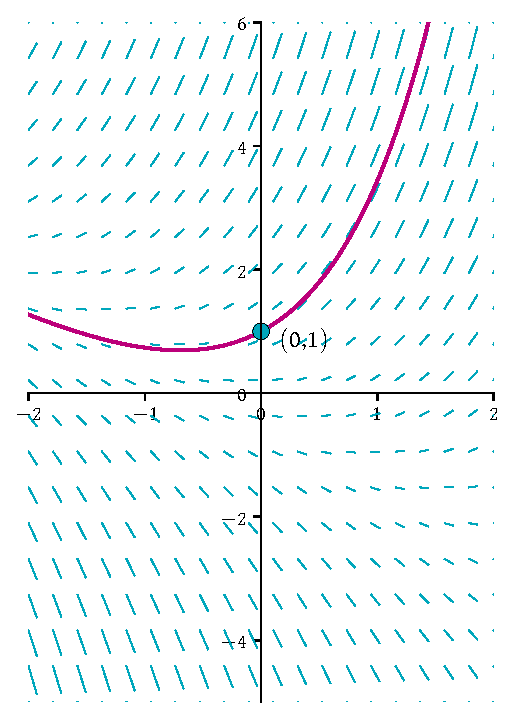
\includegraphics[width = 0.5\textwidth]{Ch3_files/Ch3_32_0.pdf}
		\caption{}
		\label{fig:direction_field}	
	\end{figure}
    
\subsection{Euler's Method}\label{eulers-method}

The basic idea behind direction fields can be used to find numerical approximations to solutions of differential equations. Take previous example, since we know the slope at the initial condition we can approximate the solution as \(y(x) = x + 1\), basically a tangent line at \((0, 1)\). Euler's method consists on improving this approximation
bit by bit and changing the direction of the slope as the direction field tells us.

So, the rough steps could be 

\begin{enumerate}
	\item Use the solution \(y(x) = x + 1\) but stop at \(x = 0.5\) (this is the \textbf{step size}). At this point, \(y(0.5) = 1.5\). 
	\item Take \((0.5, 1.5)\) as the starting point for a new line segment. The slope for this segment is \(y'(0.5) = 0.5 + 1.5 = 2\). Recall the definition of the slope of a line \(m = \frac{y - y_0}{x - x_0}\), then the solution for \(x\in[0.5,1]\) is given by 

	\[
	y = 1.5 + 2*(x-0.5) = 2x + 0.5
	\] 

	\item Iterate further taking now another initial point. In this case, \(x = 1\). If \(x = 1\), then \(y(x) = 2x +0.5 =2.5\). And the new slope is \(y'(1) = 1 + 2.5 = 3.5\).
\end{enumerate}

The key is that the smaller we make the \textbf{step size} the closer to the true solution that we will be. If we take an infinitesimal stepsize, we would be computing the slope of the solution curve for each point of the domain, and thus, computing the true solution. Obviously, this procedure by hand is tedious and very inefficient but computers are
suited for that.

We now discuss how to solve Solow's growth model using Euler's method. To recall, Solow's growth model consists of two main equations, a capital accumulation law of motion and a production function.

\paragraph{Sketch of Solow's Growth Model:} 

- Total output in the economy \((Y)\) is produced using technology, capital, and labor. Technology is
fixed and labor grows at a constant rate \(n\). The production function is \(Y = AK^{\alpha}L^{1-\alpha}\). 

- An exogenous fraction \(s\) of output is dedicated to investment and capital depreciates at constant
rate \(\delta\). Capital accumulates according to: 

\[
\dot{K} = sY - \delta K
\]

Expressing the model in terms of the capital-labor ratio \(k\), the equilibrium of the economy is given by the solution to the differential equation

\[
\dot{k} = sAk^{\alpha} - (\delta + n)k
\]

So, to solve the model, with given set of parameters \(\{A,\alpha,s,\delta,n\}\) and an initial condition \(k(0)\) we have to find the solution to previous equation. The solution is a point in which the capital-labor ratio stops growing (i.e.~the steady state). Suppose an economy starts below its steady state and it takes about 60 years to get to it. Apart from the parameters of the model, we need to choose a step-size that will tell us how often we will change the slope that determines the accumulation of capital (i.e.~\(\dot{k}\)), we choose different step sizes and see that the smaller the step size the closer the solution looks to the \emph{true} solution.

Then, given the initial condition \(k(0)\), we know that \(k(1) = k(0) + \dot{k}\). Note that we are now making two important assumptions. We are discretizing the time space, since we are computing values of the capital stock for certain \emph{years} (time is continuous, not discrete, so there are no actual years) and then, interpolate what is in between those years. Second, we are assuming a fixed step size. Obviously, doing this by hand takes a long time, but in
a computer it takes seconds. Next figure shows the solution computed with Euler's method and several step-sizes and a more efficient numerical solution implemented in Python.

\begin{figure}[htbp]
	\centering 
		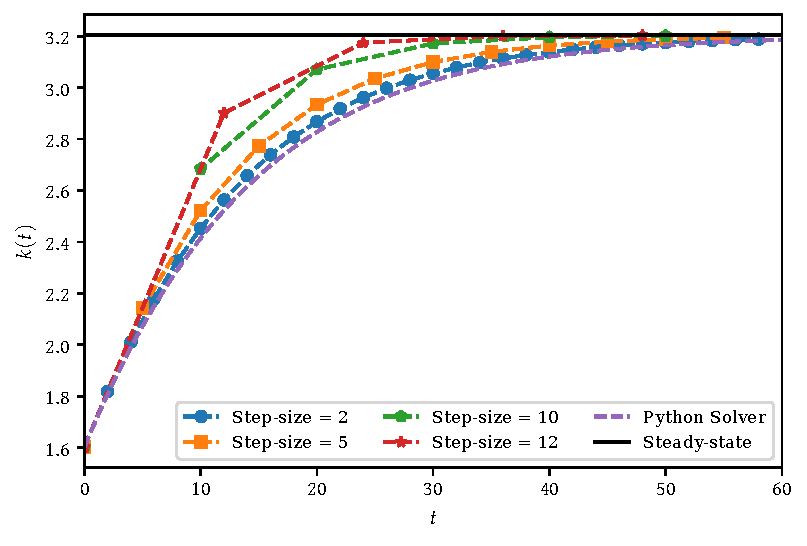
\includegraphics[width = 0.5\textwidth]{Ch3_files/Ch3_34_0.pdf}
		\caption{}
		\label{fig:solow_convergence}
\end{figure}

\section{Integration Techniques}\label{integration-techniques}

\subsection{Change of Variables}\label{change-of-variables}

An important implication of the substitution property is that we can simplify integrals significantly by applying a change of variables and undoing it later on.

\begin{example}
Compute \(\int \frac{2x}{x^2+1} dx\)

This integral is not an immediate integral but note that if we let \(z = (x^2 + 1)\), then \(dz = 2xdx\), subsituting into the integral this change of variables, we get

\[
\int \frac{2x}{x^2+1} dx = \int \frac{1}{z} dz = \ln z + \mathcal{C}
\]

To solve the integral we must undo the change of variables

\[
\int \frac{2x}{x^2+1} dx = \ln z + \mathcal{C} = \ln\left(x^2 + 1\right) + \mathcal{C}
\]
\end{example}

\begin{example}
Compute \(\int \frac{1 - \sqrt{x}}{\sqrt[3]{x}} dx\)

This is less clear than previous example, but the idea is to get rid of the square and cubic roots, to do so, note we can substitute \(x = y^6\), thus \(\sqrt{x} = y^3\) and \(\sqrt[3]{x} = y^2\). Differentiating, we get \(dx = 6y^5 dy\). Subsituting into the original integral, we need to solve now

\[
\int \frac{1 - y^3}{y^2} 6y^5 dy = \int (1 - y^3)6y^3 dy = 6 \int (y^3 - y^6) dy = 6\left(\frac{y^4}{4} - \frac{y^7}{7}\right) + \mathcal{C}
\]
\end{example}

\subsection{Integration by Parts}\label{integration-by-parts}

We stated before that integration is the inverse operation of differentiation. From differentiation rules, we know that

\[
\frac{d}{dx}\left(f(x)g(x)\right) = f'(x)g(x) + g'(x)f(x)
\]

Thus, we can integrate on both sides of this equation to get

\[
f(x)g(x) = \int f'(x)g(x) dx + \int f(x)g'(x) dx
\]

Which, rearranging we get

\begin{equation}
\int f(x) g'(x) dx = f(x)g(x) - \int g(x)f'(x) dx
\end{equation}

Which is the formula for \textbf{integration by parts}. The commonly used notation is obtained by letting now \(u(x) = f(x)\) and \(v(x) = g(x)\), then \(u'(x) = f'(x)\) and \(v'(x) = g'(x)\). By the substitution property, previous formula becomes

\[
\int u(x)v'(x) dx = u(x)v(x) - \int v(x)u'(x)dx
\]

\textbf{Tips:} To solve an integral by parts we need to choose which function will be \(u\) and which will be \(v\) some tips to choose these functions are 

\begin{itemize}
	\item Function \(u(x)\) must be differentiated to compute \(u'(x)\), which does not impose any restrictions on its choice. 

	\item We must integrate \(v'(x)\) to get \(v(x)\) thus, we want to choose \(v'(x)\) easy enough to integrate. - Note we need to compute \(\int v(x)u'(x)dx\) which needs to be easier to solve than \(\int u(x)v'(x)dx\). - Typically, it is useful to choose \(u(x)\) for polynomials or logarithms. While the choice for \(v'(x)\) is typically exponentials or trigonometric functions. When differentiating polynomials or logs, the resulting functions are easier while exponential or trigonometric functions are not simplified nor complicated after differentiating or integrating.
\end{itemize}

\begin{example}
Find \(\int x\sin x dx\)

Let \(u(x) = x\) and \(v'(x) = \sin x\). Then, \(u'(x) = 1\) and \(v(x) = \int \sin x dx = -\cos x\). Thus

\begin{align}
u(x) & = x \ & \ v'(x) = \sin x \\
u'(x) & = 1 \ & \ v(x) = -\cos x
\end{align}

\begin{align}
\int x\sin x dx & = \int u(x)v'(x)dx \\
& = u(x)v(x) - \int u'(x)v(x) dx \\
& = -x \cos x - \int (-\cos x) dx \\
& = -x\cos x + \int \cos x dx \\
& = -x \cos x + \sin x + \mathcal{C}
\end{align}
\end{example}

\begin{example}
Compute \(\int \log x dx\)

Let

\begin{align}
u(x) & = \log x \ & \ v'(x) = dx \\
u'(x) & = \frac{1}{x} \ & \ v(x) = x
\end{align}

Using the formula for integration by parts we get

\[
\int \log x dx = x\log x - \int \frac{1}{x} x dx = x\log x - \int dx = x\log x - x + \mathcal{C}
\]
\end{example}

\begin{remark}
Note that using the formula for integrating by parts and the Fundamental Theorem of Calculus we can evaluate definite
integrals by parts.
\end{remark}

\section{Improper Integrals}\label{improper-integrals}

When we have talked about definite integrals, we were using functions \(f(x)\) defined on a finite interval \([a, b]\) where \(f(x)\) does not have infinite discontinuities in that interval. We can extend the concept of definite integrals for the case where the interval is infinite or we have infinite discontinuities in the interval \([a, b]\).
These types of integrals are called \emph{improper} integrals, you will see a great deal of them all over economics, econometrics, probability\(\ldots\)

\subsection{Type I: Infinite Intervals}\label{type-i-infinite-intervals}

Consider the function \(f(x) = 1/x^2\) above the \(x-\)axis and to the right of \(x = 1\). Figure \ref{fig:improper_type1} shows the function and the area we want to compute. The highlighted area can be formally expressed as the integral

\[
A(t) = \int^t_1 \frac{1}{x^2} dx = -\frac{1}{x}\Bigg]^t_1 = 1 - \frac{1}{t}
\]

For whatever \(t\) we choose. Note that \(A(t)\) is always less than \(1\) since \(t>1\). Further note that the limit of \(A(t)\) for \(t\rightarrow\infty\) is equal to \(1\), so the area approaches \(1\) as \(t\) goes to infinity. We can then write

\[
\int^{\infty}_1 \frac{1}{x^2} dx = \lim_{t\rightarrow\infty}\int^t_1\frac{1}{x^2} dx = 1
\]

\begin{figure}[htbp]
	\centering 
		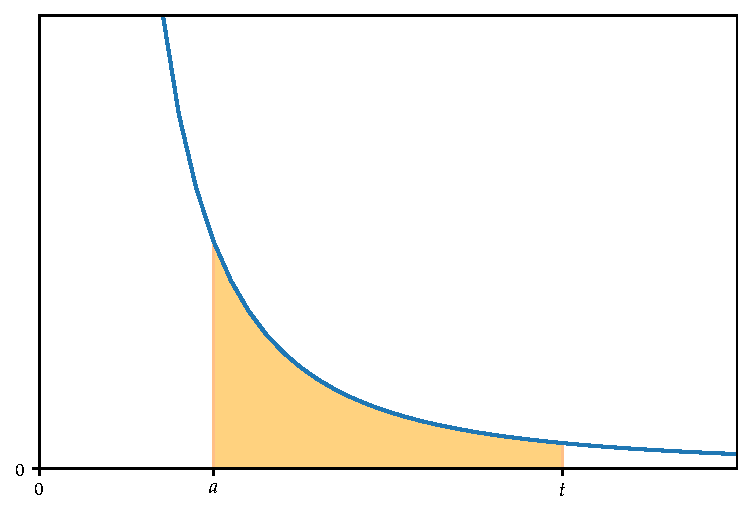
\includegraphics[width=0.6\textwidth]{Ch3_files/Ch3_38_0.pdf}
		\caption{}
		\label{fig:improper_type1}
\end{figure}

\begin{definition}
An improper integral of Type I: 

\begin{enumerate}
	\item If \(\int^t_a f(x) dx\) exists \(\forall t\geq a\), then

	\[
	\int^{\infty}_a f(x) dx = \lim_{t\rightarrow\infty}\int^t_a f(x) dx
	\]

	provided this limit exists.
	\item  If \(\int^b_t f(x) dx\) exists \(\forall t\leq b\), then

	\[
	\int_{-\infty}^b f(x) dx = \lim_{t\rightarrow -\infty}\int^b_t f(x) dx
	\]

	provided this limit exists.
\end{enumerate}

These improper integrals are \textbf{convergent} if the corresponding limit exists and \textbf{divergent} otherwise.

If both \(\int^{\infty}_a f(x) dx\) and \(\int_{-\infty}^b f(x) dx\) are convergent, then

\[
\int_{-\infty}^{+\infty} f(x) dx = \int_{-\infty}^c f(x) dx + \int^{\infty}_c f(x) dx \ \forall \ c\in\mathbb{R}
\]
\end{definition}

\subsubsection{Type II: Discontinuous Integrands}\label{type-ii-discontinuous-integrands}

Suppose \(f(x)\) is a positive continuous function defined on a finite interval \((a,b]\) but has a vertical asymptote at \(x=a\). Let \(S\) be the region bounded under the graph of \(f(x)\) and above the \(x-\)axis in \((a,b]\), in this case the region extends infinitely in a vertical direction (Figure \ref{fig:improper_type2} shows this). The area of \(S\) between \(a\) and \(t\) is

\[
A(t) = \int^b_t f(x) dx
\]

If we have that \(A(t)\) approaches a definite number as \(t\rightarrow a^{+}\), we say tht the area of the region \(S\) is \(A\) and we write

\[
\int^b_a f(x) dx = \lim_{t\rightarrow a^{+}} \int^b_t f(x) dx
\]

\begin{figure}[htbp]
	\centering 
		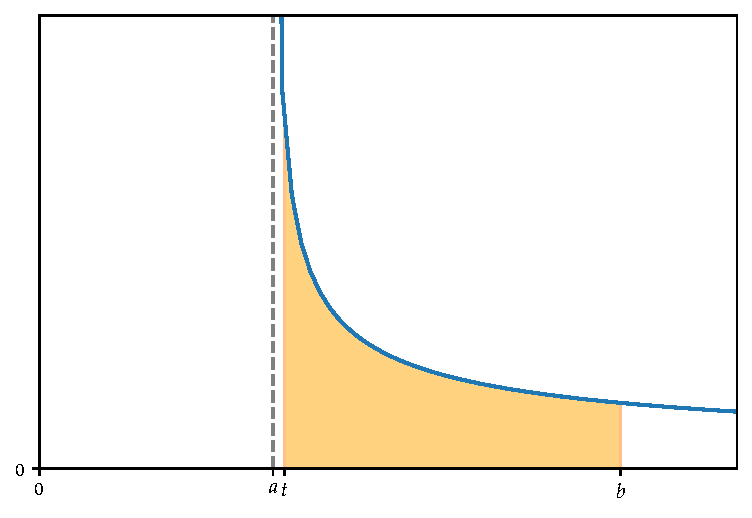
\includegraphics[width = 0.6\textwidth]{Ch3_files/Ch3_41_0.pdf}
		\caption{}
		\label{fig:improper_type2}
\end{figure}

\begin{definition}
An improper integral of Type II: 

\begin{enumerate}
	\item If \(f(x)\) is continuous on \([a,b)\) and is discontinuous on \(b\), then

	\[
	\int^{b}_a f(x) dx = \lim_{t\rightarrow b^{-}}\int^t_a f(x) dx
	\]

	provided this limit exists.

	\item If \(f(x)\) is continuous on \((a,b]\) and is discontinuous on \(a\) then
	
	\[
	\int^{b}_a f(x) dx = \lim_{t\rightarrow a^{+}}\int^b_t f(x) dx
	\]

	provided this limit exists.
\end{enumerate}

The improper integral \(\int^b_a f(x) dx\) is called \textbf{convergent} if the corresponding limit exists and \textbf{divergent} if the limit does not exist.

If \(f(x)\) has a discontinuity in \(c\in[a,b]\) and both \(\int^c_a f(x) dx\) and \(\int^b_c f(x) dx\) are convergent, then we define

\[
\int_{b}^{a} f(x) dx = \int_{a}^c f(x) dx + \int^{b}_c f(x) dx
\]
\end{definition}

\section{Sequences and Series}\label{sequences-and-series}

\subsection{Definition of a Sequence}
\begin{definition}
A sequence of real numbers is a rule that assigns to each natural number $n\in \mathbb{N}$ a real number $a_n$.

\[
\{a_n\}
\]

First term $a_1$, second term $a_2$,$\ldots$, $n-$th term $a_n$. More formally, a sequence is a function that maps the natural numbers into $\mathbb{R}$, that is

\[
a : \mathbb{N} \mapsto \mathbb{R}, \ n \mapsto a_n
\]
\end{definition}

\begin{align*}
& a_n = n & \ & a_1=1, a_2=2,  a_3=3,  a_4 = 4,  \ldots \\ 
& a_n = \dfrac{1}{n} & \ & a_1=1, a_2=\dfrac{1}{2},  a_3=\dfrac{1}{3},  a_4 = 
\dfrac{1}{4},  \ldots \\
& a_n= \dfrac{n+1}{n} & \ & a_1=2, a_2=\dfrac{3}{2},  a_3=\dfrac{4}{3},  a_4 = 
\dfrac{5}{4},  \ldots \\
& a_n = 2^n & \ & a_1=2, a_2=4,  a_3=8,  a_4 = 16,  \ldots \\
& a_n = \left( \dfrac{1}{3} \right)^n & \ & a_1=\dfrac{1}{3}, a_2=\dfrac{1}{9},  
a_3=\dfrac{1}{27},  a_4 = \dfrac{1}{81},  \ldots \\
& a_n = (-1)^n & \ & a_1=-1, a_2=1,  a_3=-1,  a_4 = 1,  \ldots \\
\end{align*}

\begin{definition}
We say a sequence $\{a_n\}$ \textbf{converges} to the limit $\mathcal{L}$ if 

\[
\forall \varepsilon > 0 \ \exists n_0 \in \mathbb{N} \text{ such that } n\geq n_0, \text{ then } \lvert a_n - \mathcal{L} \rvert < \varepsilon
\]

Which can be written as

\[
\mathcal{L} = \lim_{n\rightarrow\infty} a_n
\]
\end{definition}


\begin{definition}
A sequence $\{a_n\}$ is said to be \textbf{geometric} if the relationship between any two consecutive terms is always constant:

\[
\frac{a_{n+1}}{a_n} = r \ \forall n\in\mathbb{N}
\]

The constant $r$ is called the \textit{common ratio of the geometric sequence}. Then, any geometric sequence can be written as follows:

\[
a_0 = A, a_1 = Ar, \ldots, a_n = Ar^n, \ldots
\]
\end{definition}

\begin{lemma}
A geometric sequence with common ratio $r$ is convergent if $r\in (-1,1]$ and it is divergent otherwise.
\end{lemma}

\begin{proof}
Five cases can be distinguished:
\begin{itemize}
	\item If $r = 1$, the sequence is constant, $a_n = A$ for every $n\in\mathbb{N}$, thus its limit is $L = A$ and the sequence is convergent.
	\item If $r = -1$ the sequence is $a_1 = -A, a_2 = A, a_3 = -A, a_4 = A, \ldots$ thus it is oscillating between these two values and does not approach any limit. Thus, the sequence is divergent.
	\item If $-1 < r < 1$, when computing $r^n$ a smaller number in absolute value is obtained each time, which becomes as small as wished. Thus, its limit is $L = 0$ (regardless of the value of $A$) and the sequence is convergent.
	\item If $r\in (1,+\infty)$, then $r^n$ grows and tends to $+\infty$. Thus, the sequence is divergent.
	\item If $r\in(-\infty, -1)$, then when computing powers (even powers will be positive, odd ones will be negative) very large numbers are obtained in absolute value (as large as wished). Thus, the sequence is divergent
\end{itemize}
\end{proof}

\subsection{Definition of Series}

\begin{definition}
Let \(\{a_n\}\) be a sequence of real numbers. Then, the associated \textbf{series} is defined as the ordered formal
sum

\[
\sum^{\infty}_{n=1} a_n = a_1 + a_2 + a_3 + \ldots
\]
\end{definition}

\begin{definition}
The sequence of \textbf{partial sums} associated to the series \(\sum^{\infty}_{n=1}a_n\) is defined as

\[
S_n = \sum^n_{i=1} a_i \text{ for } n\in\mathbb{N}
\]
\end{definition}
The series converges 
to a limit \(\mathcal{S}\) if the sequence \(S_n\) converges to \(S\), i.e.

\[
S = \sum^{\infty}_{i=1} a_i \text{ if and only if } S = \lim_{n\rightarrow\infty} S_n = \lim_{n\rightarrow\infty}\sum^n_{i=1} a_i
\]

Otherwise, it is called \textbf{divergent}.

To see whether a series is convergent or not, we state and prove a \textbf{necessary} (not sufficient) condition for convergence of a series.

\begin{theorem}
If the series \(\sum^{\infty}_{n=1} a_n\) is convergent, then \(\lim_{n\rightarrow\infty}a_n = 0\).
\end{theorem}

\begin{proof}
It is sufficient to note that

\[
a_n = S_{n} - S_{n-1}
\]

Since

\[
\lim_{n\rightarrow\infty}S_{n} = \lim_{n\rightarrow\infty}S_{n-1} = S \Rightarrow \lim_{n\rightarrow\infty}a_{n} = S - S = 0
\]
\end{proof}

\begin{example}
The sequence \(a_n = \dfrac{1}{n}\) is convergent, since \(\lim_{n\rightarrow\infty} \dfrac{1}{n} = 0\). However, the
series

\[
\sum^{\infty}_{i=n} \frac{1}{n}
\]

is divergent.
\end{example}

We have seen that the geometric sequence converges if and only if \(\lvert r \rvert <1\), it turns out that the same holds true for the associated geometric series.


\begin{theorem}
The \emph{geometric series} converges if and only if \(\lvert r\rvert < 1\) and

\[
A\sum^{\infty}_{n=0} r^n = A\frac{1}{1-r}
\]
\end{theorem}

\begin{proof}
Note that

\begin{align*}
S_n(1-r) = S_n - rS_n &= A\sum^n_{k=0}r^k - Ar\sum^{n}_{k=0} r^k = A\left(\sum^n_{k=0} r^k - \sum^n_{k=0} r^{k+1}\right) \\
&= A\left(\sum_{k=0}^n r^k - \sum^{n+1}_{k=1} r^k\right) =A\left( r^0 - r^{n+1}\right) = A\left(1-r^{n+1}\right)
\end{align*}

Thus,

\[
S_n = \frac{A\left(1-r^{n+1}\right)}{1-r}
\]

Now, computing the limit of \(S_n\), we can see

\[
\lim_{n\rightarrow\infty} S_n = \lim_{n\rightarrow\infty} \frac{A\left(1-r^{n+1}\right)}{1-r} = \frac{A\left(1 -  \displaystyle\lim_{n\rightarrow\infty} r^{n+1}\right)}{1-r} =  \frac{A}{1-r} \text{ if and only if }\lvert r \rvert < 1
\]
\end{proof}

\section{Taylor Expansion}\label{taylor-expansion}

A very useful series used \textbf{a lot} in macroeconomics (wait until you see a log-linearization of a DSGE model) is the Taylor Expansion. Let us define it now.

\begin{definition}
The \textbf{Taylor polynomial} of order \(n\) of a function \(f(x)\) which is \(n\) times differentiable around a point
\(x = a\) is given by

\[
P_n\left(f,a\right) = f(a) + \frac{1}{1!}f'(a)(x-a) + \frac{1}{2!} f''(a)(x-a)^2+\ldots+\frac{1}{n!}f^{(n)}(a)(x-a)^n
\]

When \(a = 0\), it is called \textbf{McLaurin Polynomial}.
\end{definition}

When the Taylor expansion is for \(n\rightarrow\infty\) a power series arises as

\[
S\left(f,a\right) = f(a) + \sum^{\infty}_{n=1} \frac{1}{n!}f^{(n)}(a)(x-a)^n
\]

The following theorem tells us that the Taylor expansion of any infinite-times differentiable function coincides with the actual value of the function around that point. Thus, an n-degree approximation of a function can be a very good approximation.

\begin{theorem}
If the derivatives of any order of a function \(f(x)\) exist in a point \(x = a\), then

\[
f(x) = f(a) + \sum^{\infty}_{n=1} \frac{1}{n!}f^{(n)}(a)(x-a)^n \ \forall x\in(a-\delta,a+\delta)
\]

Where \(\delta>0\) but small.
\end{theorem}


\section{Exercises}\label{exercises}

\begin{enumerate}
	\item Let \(f(x)\) and \(g(x)\) be two functions such that \(f'(x) = g'(x)\). Is it true that \(f(x) = g(x)\)? In case it is true, prove it. If it is not, it is sufficient to show a counterexample.

	\item Compute \(f(x)\) knowing that \(f'(x) = x^2 - 3x + 5\) and \(f(0) = 1\).

	\item Solve the differential equation \(y'(t) = \frac{-2t}{y(t)}\) with the initial condition \(y(0) = 1\). Plot its solution.

	\item Prove that the repeating decimal \(0.9999\ldots\) is equal to \(1\).

	\item Compute the steady state in the Solow model studied above (i.e. note that in the graph the steady state is a constant, find out what the value of that constant is).

	\item Compute the \textbf{area} of the region bounded by \(f(x) = x^2-1\) and \(g(x) = 4x-4\) for \(x\in[0, 4]\)
	
	\item Study the limit of the sequence \(\lim_{n\rightarrow\infty}\left(-\frac{1}{2}\right)^{n}\).

	\item Compute the integral \(\int^{+\infty}_{-\infty} f(x)dx\) where
	
	\[
	f(x) = \begin{cases}
	e^x & \text{if } x\leq 0 \\
	e^{-x} & \text{if } x > 0
	\end{cases}
	\]
\end{enumerate}
\end{document}